% \textbf{Title: Frequency Domain 2}

Consider a function with this spectrum.

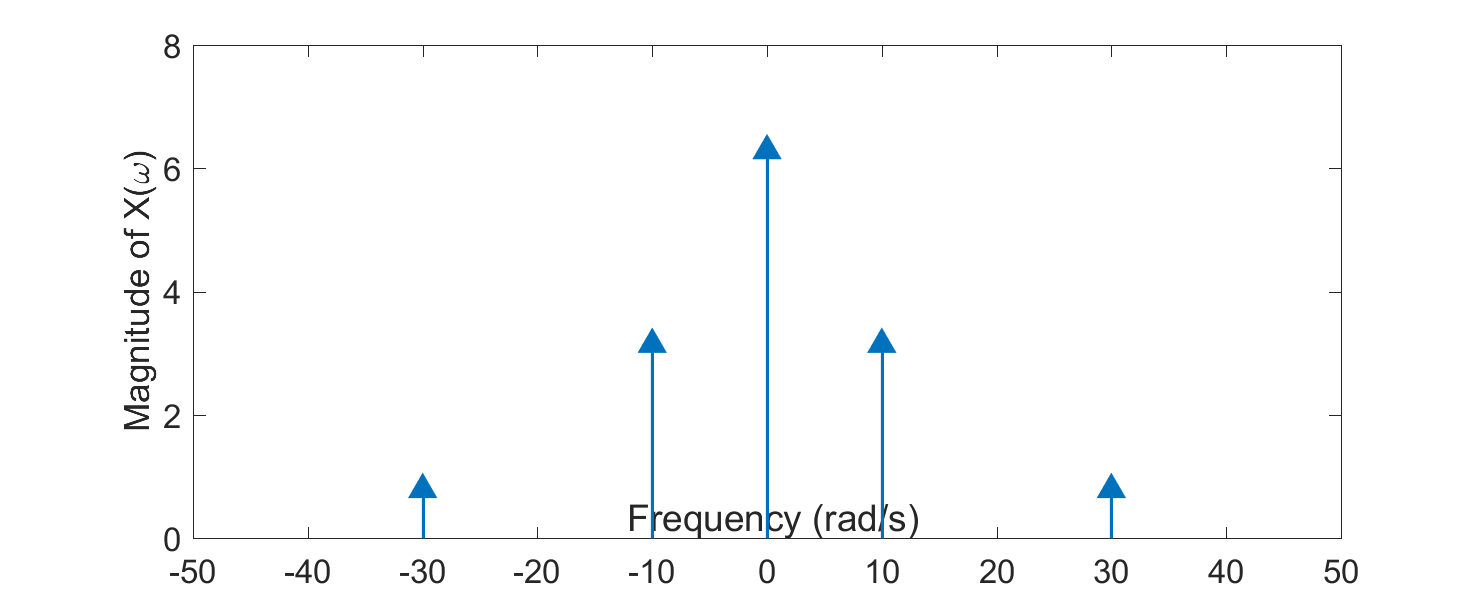
\includegraphics[width=4.52749in,height=1.84565in]{../../Images/FrequencyDomainQ2Spectr.png}

What will the spectrum of this function be if we convolve this function with \(\frac{15}{2\pi}\text{rect}\left( \frac{15t}{2\pi} \right)\)?

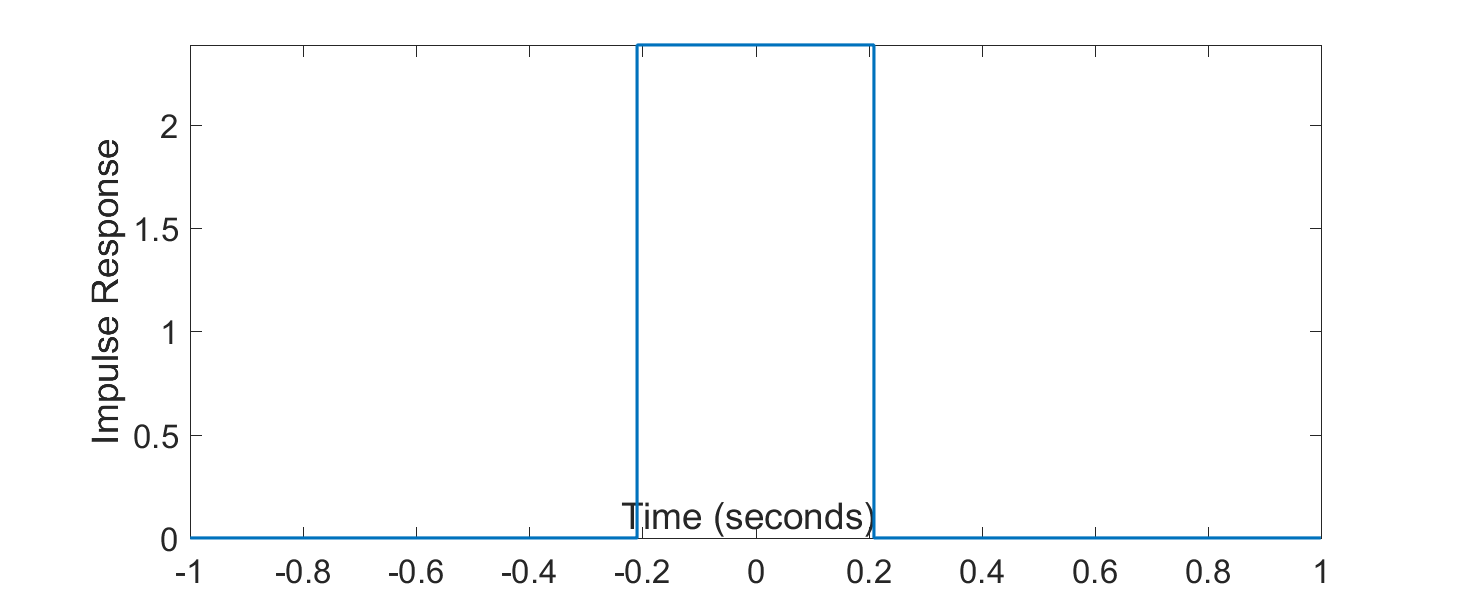
\includegraphics[width=4.5in,height=1.5in]{../../Images/FrequencyDomainQ2Conv.png}\\

a. 

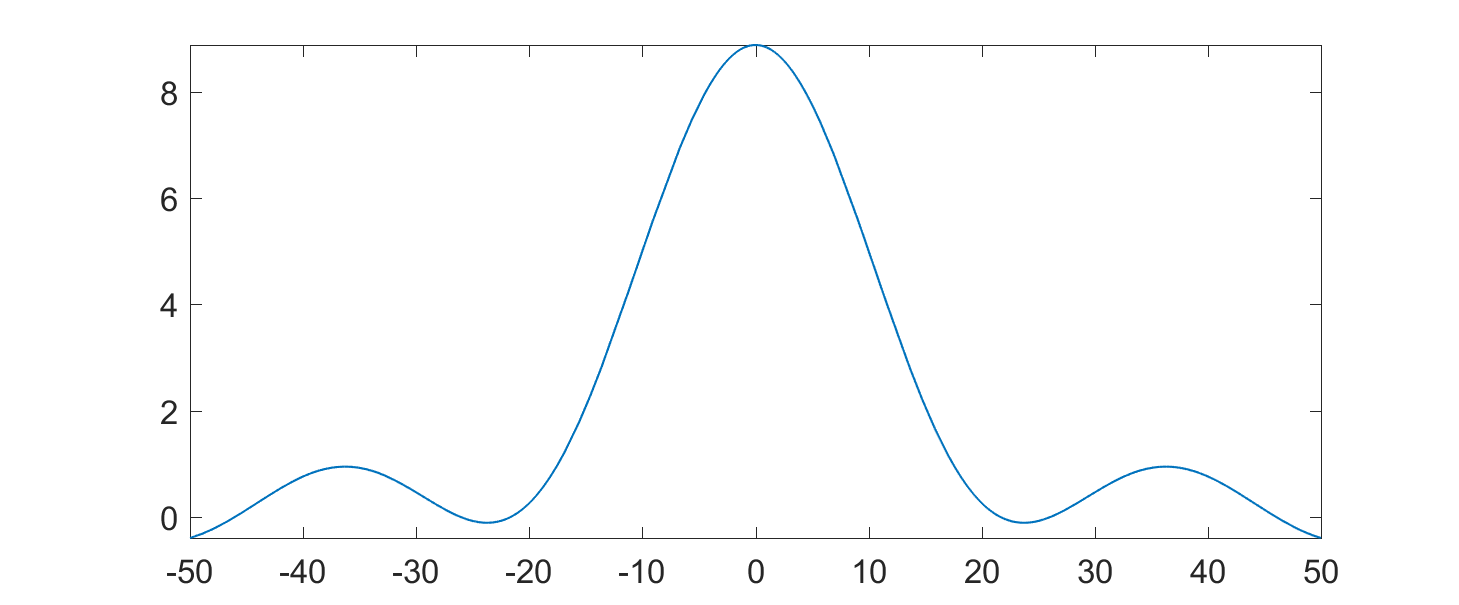
\includegraphics[width=4.5in,height=1.5in]{../../Images/FrequencyDomainQ2a.png}

b. 

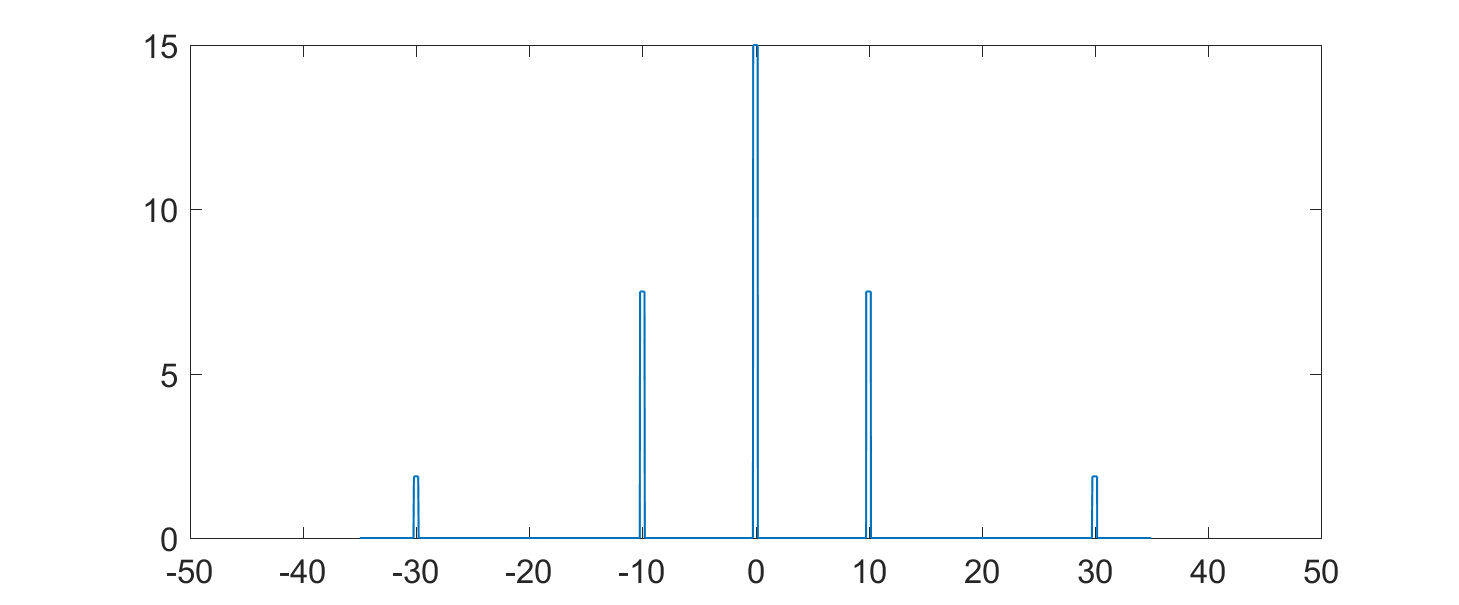
\includegraphics[width=4.5in,height=1.5in]{../../Images/FrequencyDomainQ2b.png}

c. 

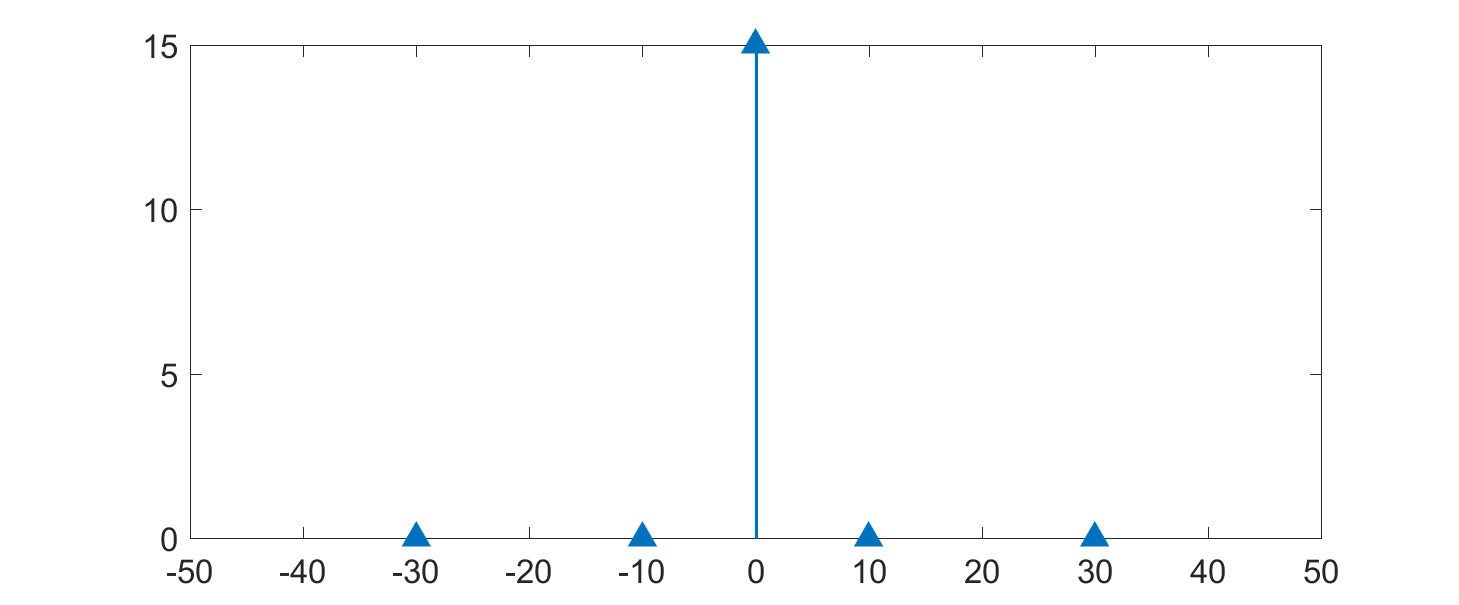
\includegraphics[width=4.5in,height=1.5in]{../../Images/FrequencyDomainQ2c.png}

*d.

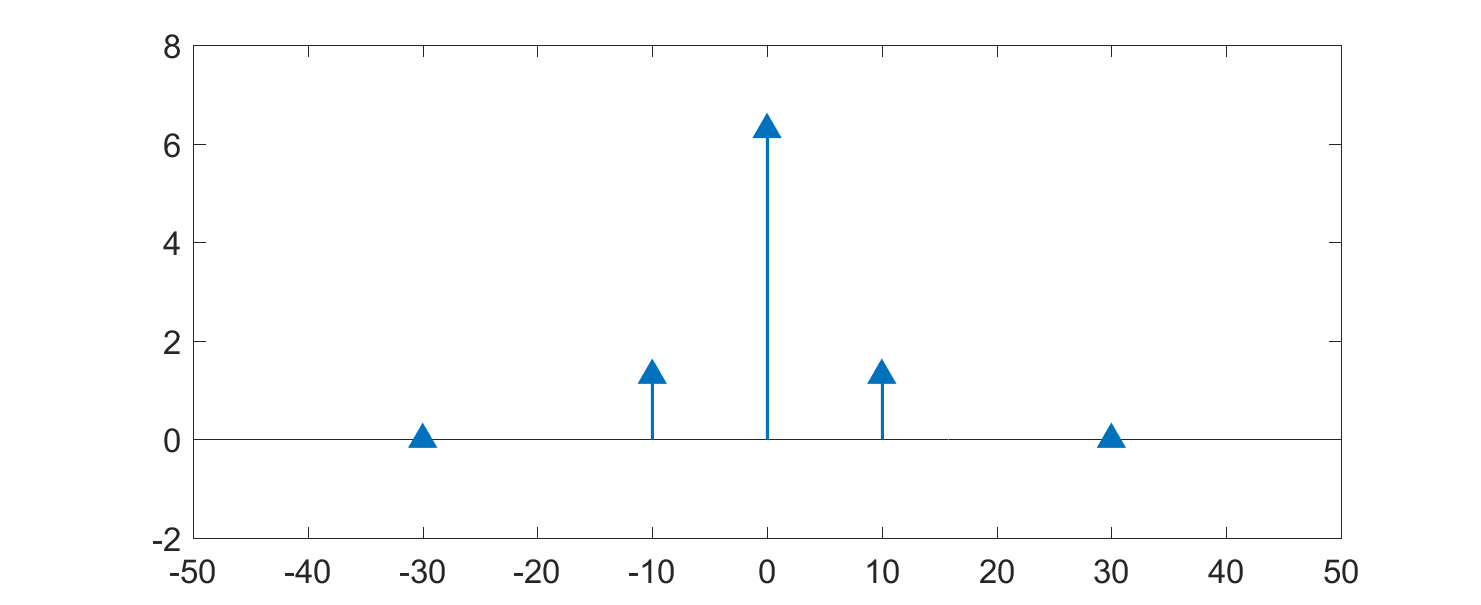
\includegraphics[width=4.5in,height=1.5in]{../../Images/FrequencyDomainQ2d.png}

e. 

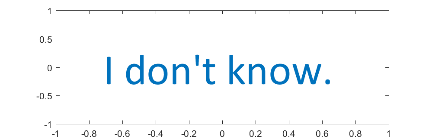
\includegraphics[width=1.92042in,height=0.62319in]{../../Images/AnswerEGraph.png}\\
